\documentclass[titlepage,a4paper]{jsarticle}
\usepackage{../sty/import}% 各種パッケージインポート
\usepackage{../sty/title_team}% タイトルページの変更

%% タイトルページの変数
% レポートタイトル
\title{Driving-saver仕様報告書}
% 提出日
\expdate{\today}
% 科目名
\subject{マルチメディア情報論}
% 分野
\class{情報経営システム工学分野}
% 学年
\grade{B3}
% 学籍番号
\mynumber{24336488}
% 記述者
\author{本間三暉}
% グループ名 % もし班があるやつならtitle_team.styを入れる
\team{A}
% 共同実験者 % もし共同実験者が必要なやつならtitle_kyoudou.styを入れる
\coauthor{%
 \textbf{学籍番号:}24332587 & \textbf{氏名:}浅見圭祐  \\
 \textbf{学籍番号:}24332990 & \textbf{氏名:}内田晴己  \\
 \textbf{学籍番号:}24333290 & \textbf{氏名:}小笠原優心 \\
 \textbf{学籍番号:}24336684 & \textbf{氏名:}松浦瑛太  \\
}
%
% 記載例:
%\coauthor{%
% 学籍番号:24567321 & 氏名:吉田 富美男 \
% 学籍番号:12345678 & 氏名:安藤 雅洋 \
% 学籍番号:13579234 & 氏名:雲居 玄道 \
%%

\begin{document}
% titleページ作成
\maketitle
\section{はじめに}
自動車安全運転センターの初心運転者の運転意識と実態に関する調査研究\cite{自動車}によると,
年間の交通事故の10人に1人以上が運転免許取得後1年未満の運転初心者である.

運転初心者は車幅感覚が身についていないことや,道路に慣れておらず正しい道の選択ができないことが原因としてあげられる.
これは,教習所の講習だけでは運転に必要な感覚が全て身につかないからではないかと考えられる.

昨今ADSD(先進運転システム)を搭載した自動車が開発・製造されている.
しかし,ADSDを搭載した車は高く,運転免許を取り立ての10代20代の経済力では手を出しにくい.

そこで,私達はADSDよりも手軽なアプローチとして運転初心者の人間が危険な道に入って事故を起こすのを防止することを目的として,
Driving-saverというシステムを提案する.
Driving-saverは車内カメラと専用マップアプリを用いて運転中に危険を通知する.
車内カメラを用いて車幅間隔を計測し,道路端とある一定以上近づいたら運転者に音で警告する.
また,そうやって集めたデータを用いて事故の起きやすい場所をマップ上に表示する.
\section{実現方法の検討}
実現方法について検討する.
\subsection{システムの全体構成}
システムの全体をユースケース図に起こしたものを図\ref{ユースケース図}に,シーケンス図に起こしたものを図\ref{シーケンス図}に,
ER図に起こしたものを図\ref{ER図}に,クラス図に起こしたものを\ref{クラス図}に示す.

\begin{figure}[H]
  \centering
  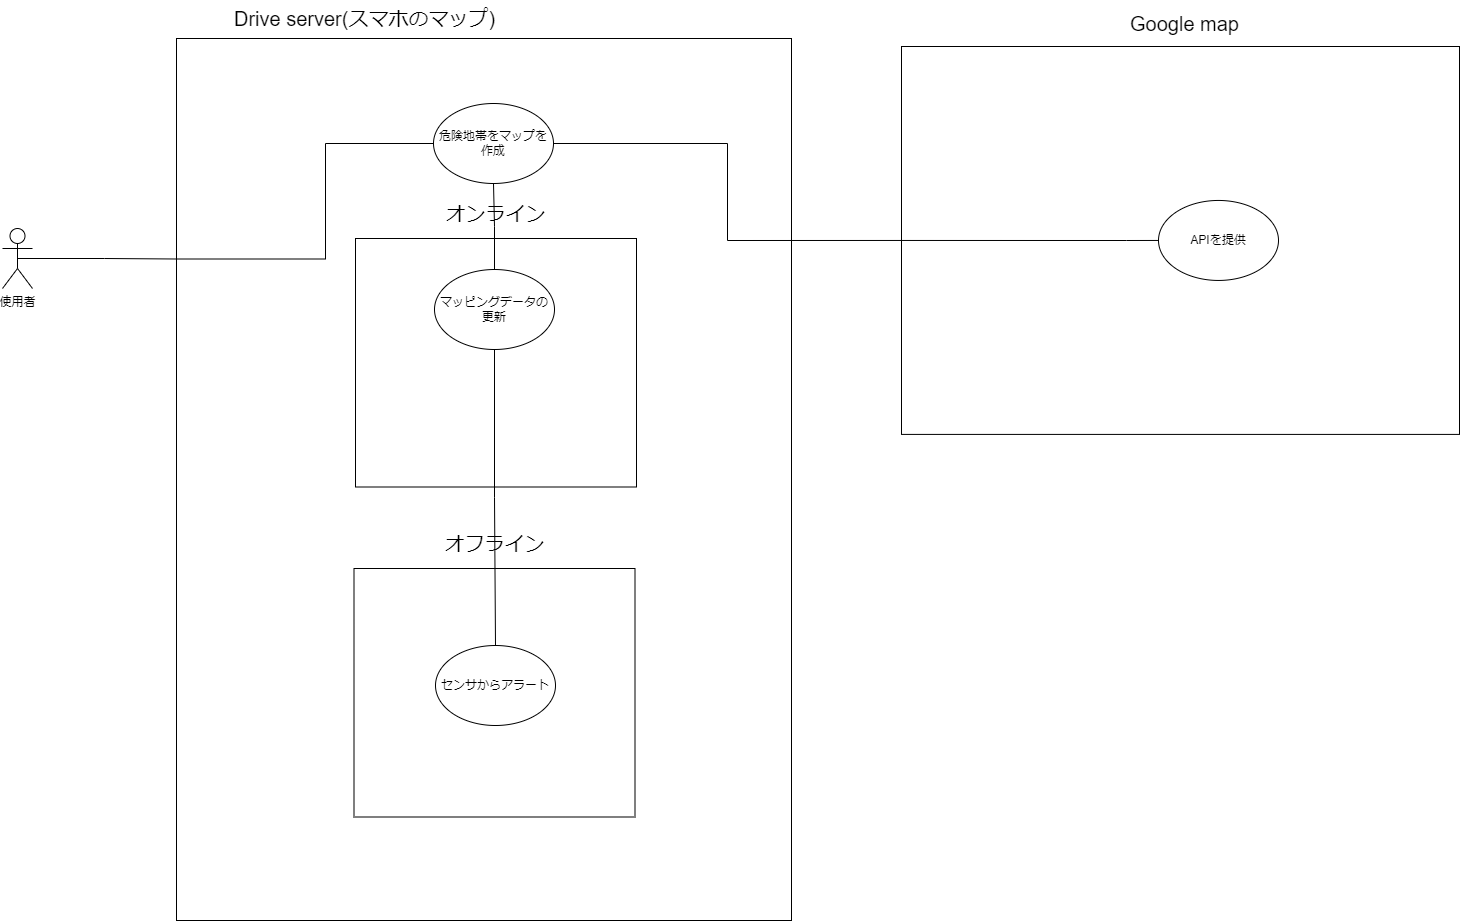
\includegraphics[width=\textwidth]{img/usecase.drawio.png}
  \caption{ユースケース図}
  \label{ユースケース図}
\end{figure}

\begin{figure}[H]
  \centering
  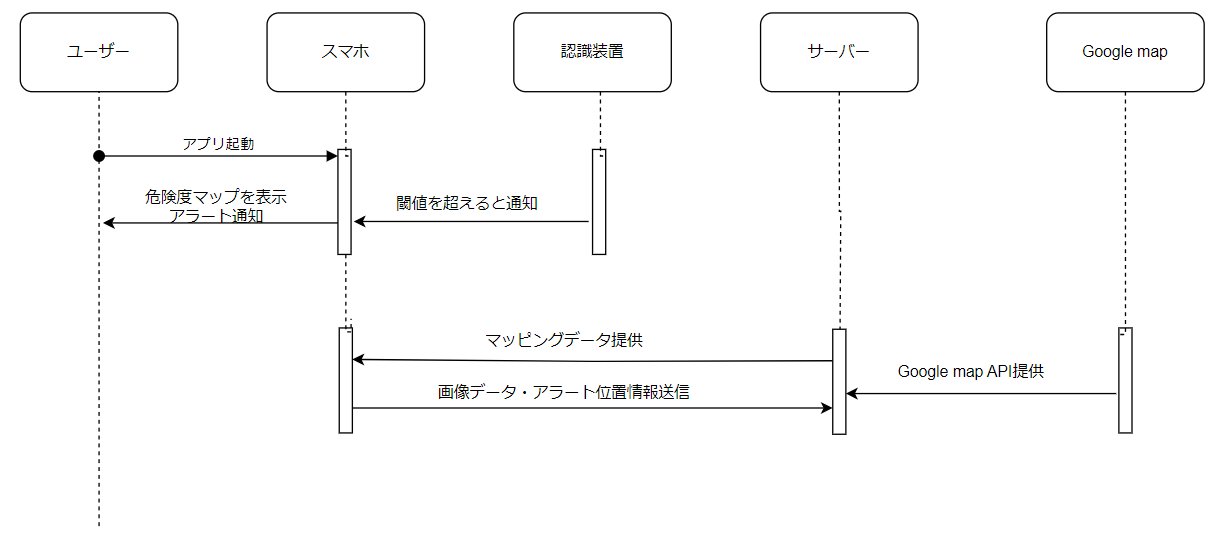
\includegraphics[width=\textwidth]{img/sea_fig.png}
  \caption{シーケンス図}
  \label{シーケンス図}
\end{figure}

\begin{figure}[H]
  \centering
  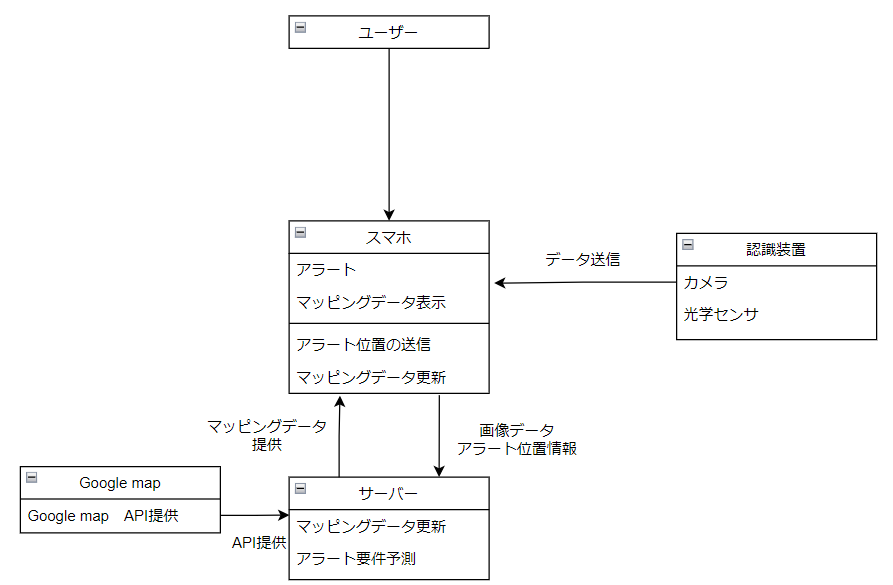
\includegraphics[width=\textwidth]{img/class_fig.png}
  \caption{クラス図}
  \label{クラス図}
\end{figure}

\begin{figure}[H]
  \centering
  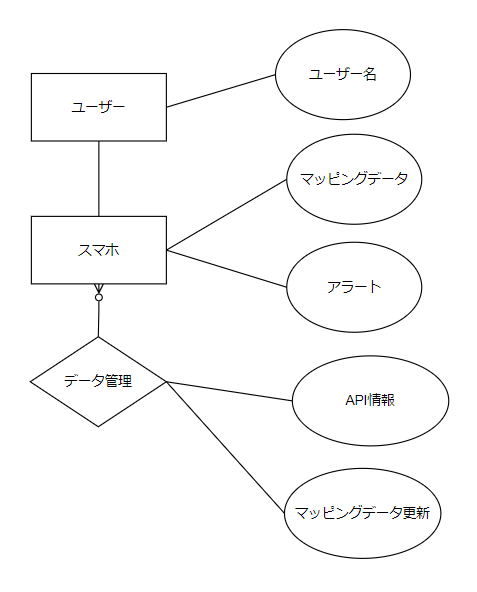
\includegraphics[width=\textwidth]{img/ER_fig.png}
  \caption{ER図}
  \label{ER図}
\end{figure}

構成要素はデバイスとソフトウェア,データベースの3つに分けられる.
\subsection{各構成要素の機能}\label{構成要素}
デバイスは赤外線カメラ2台とスマートフォンを用いる.
赤外線カメラはカメラ機能と赤外線カメラ機能を持つもので,Bluetooth,自動ピント調整機能を持ち,画像データをスマートフォンに送信する.

スマートフォンでは,後述のマップアプリを実行し,Wi-fi等を用いてサーバーと接続する.
また,カメラとはBluetoothを用いて接続する.

マップアプリでは,現在位置周辺のマップを表示する.
この時,サーバーからマップデータを受信し受信したマップデータを表示する.
表示されたマップ上にはあまり多くの車が通っていない場所や,
事故が多発している場所のような危険エリアが表示されている.
また,機械学習モデルを用いてスマートフォンと接続したカメラの入力画像の処理を行い,
国道や県道のような白線読み取りが可能な場所であれば白線認識を,農道や獣道など不可な場所であれば立体認識AIを用いて現在の走行位置を割り出し,
正しくキープレフト走行ができていなければアラートを鳴らす.

これらの機能により初心者に今よりも安全な運転をできるのではないかと考えている.
\subsection{通信方法}
節\ref{構成要素}でも挙げた通り,マップアプリを実行しているスマートフォンはWi-fi等を用いてサーバーと接続しカメラとはBluetoothを用いて接続する.
\subsection{一連の流れ}
ナビゲート開始時に,カメラモジュールを起動し,画像データの取得を開始すると共にスマートフォンとBluetooth接続し画像データの受診を行う.
また,スマホはサーバーと通信を開始し,マップデータを更新する.

ナビゲートを行っている際の危険感知をした際のアラートはスマートフォンから行う.
また,走行時の画像データや位置情報などはWi-fiなどを通じてデータベースへ送信する.

最後に,ナビゲート終了時に,カメラモジュールとスマートフォンの接続を切り,カメラモジュールを停止させる.
また,サーバーとの通信を終了し,最終マップデータを保存する.
\section{各要素の設計}
\subsection{利用する部品・モジュール}
利用する部品・モジュールと参考にしたサイトを示す.
\begin{itemize}
  \item Raspberry Pi Zero W(0.75W)\cite{ラズパイ}:カメラモジュールとスマートフォンをBluetooth接続
  \item Raspberry Pi Camera V3 Wide NoIR 赤外線(2W)\cite{ラズパイ} $\times$ 2:カメラモジュール
  \item カーチャージャー(24W)\cite{カーチャージャー}:電源供給
\end{itemize}
合計で19040円ほどとなっており,安価で実装できる事がわかる.
\subsection{ハードウェア}
図\ref{ハードウェア}に示すようにカメラモジュールを取り付ける.
\begin{figure}[H]
  \centering
  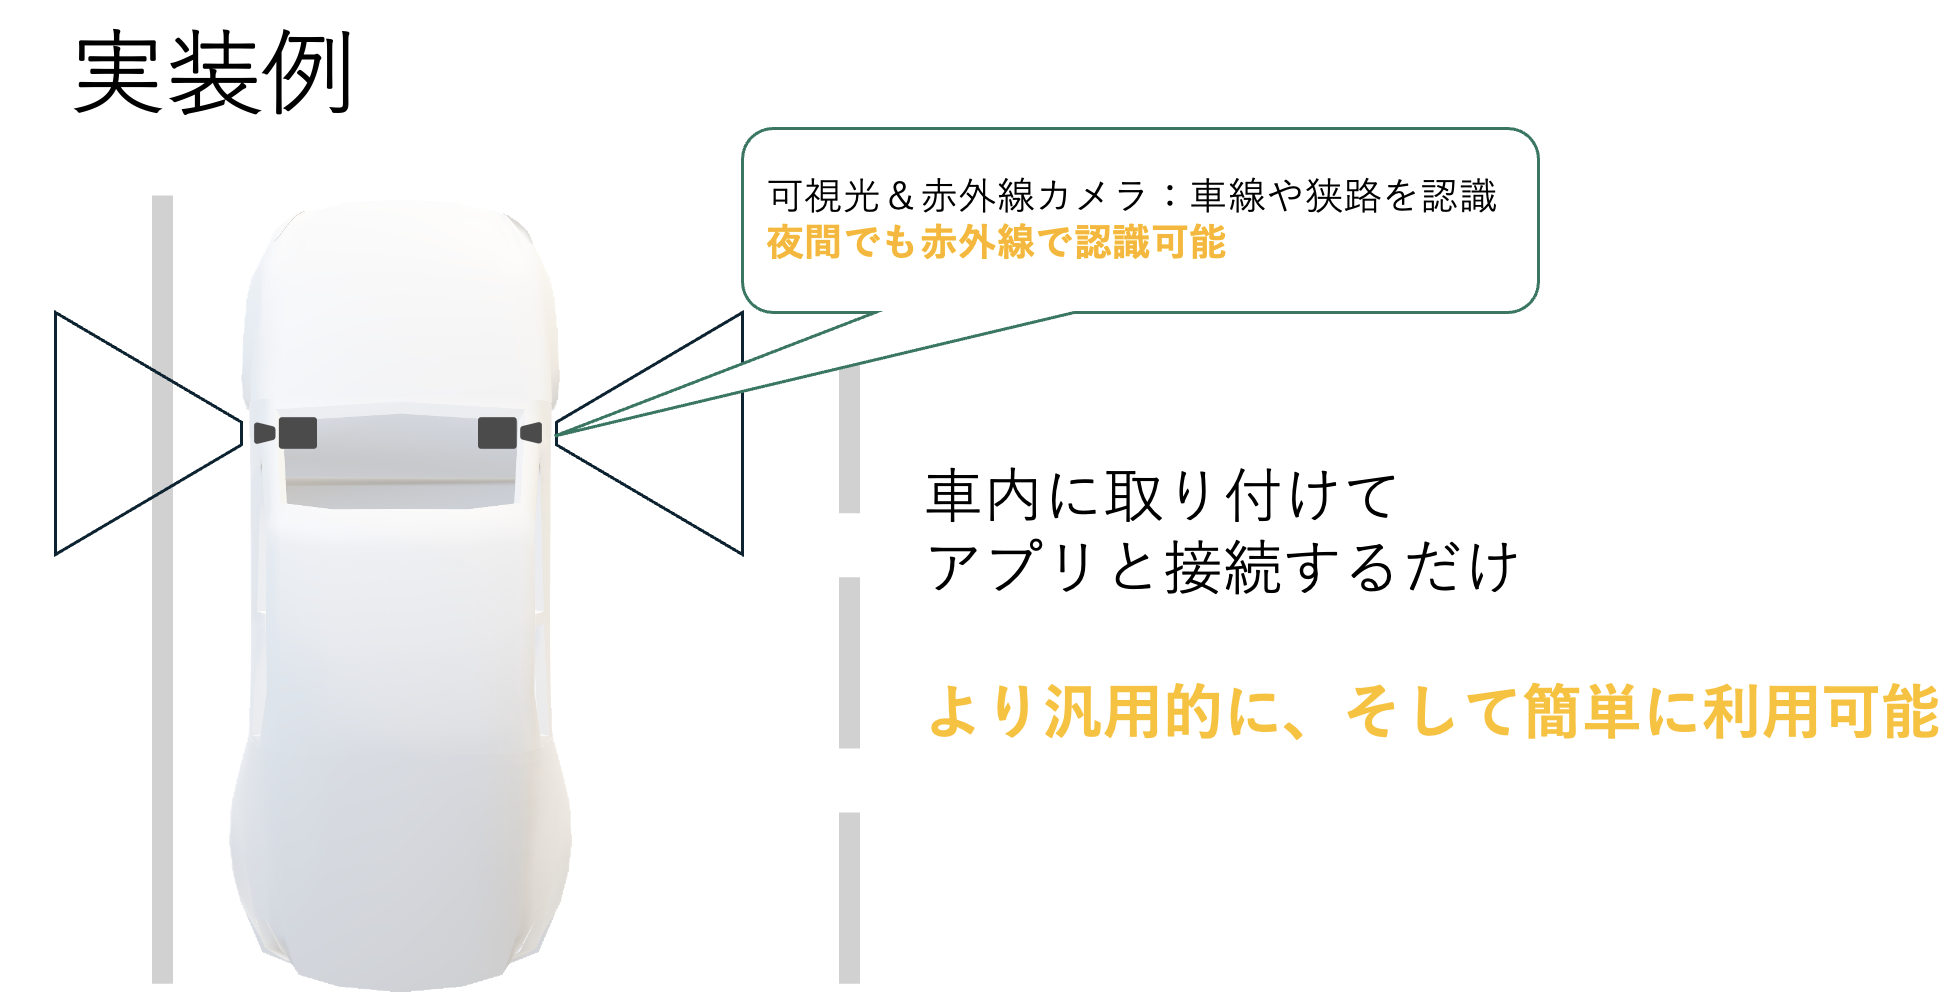
\includegraphics[width=0.8\textwidth]{img/hardware.png}
  \caption{実装例}
  \label{ハードウェア}
\end{figure}

\subsection{ソフトウェア}
Google APIを用いてマップデータを読み込む.
また,スマートフォンで白線認識\cite{白線}や立体認識AI\cite{立体認識}を実行する.

\section{ビジネスモデル}
ビジネスモデルとして,サービス全体のサブスクリプションを提案する.
サブスクリプションの登録時にハードウェアを貸与することで初期導入コストを最小限に抑えることができ,
充分なユーザー数の確保ができると考えられる.

\section{今後の展望}
使うことができるセンサが限られるため崖や雪道などに対応しきれないという問題点がある.
対応策として,前方にカメラモジュールを追加することで,より高精度な画像認識を行えるようにする.
みちびきという準天頂衛星システムやLiDARスキャナなどの技術を使った上位モデルの開発を行い,ユーザの選択肢を増やす.
高性能センサの低価格化を待つことで値段を据え置きでより高性能なモデルの開発などを考えている.

% 参考文献
\begin{thebibliography}{99}
  \bibitem{自動車} 「初心運転者の運転意識と実態に関する調査研究」自動車安全運転センター\\% 前提
  \url{https://www.jsdc.or.jp/Portals/0/pdf/library/research/h02_1.pdf}
  \bibitem{ラズパイ} Raspberry Pi Shop by KSY\\
  \url{https://raspberry-pi.ksyic.com/main/index}
  \bibitem{カーチャージャー}Amazon.co.jp: エレコム カーチャージャー シガーソケット 24W (1ポート最大12W) USB-A ×2
  【 iPhone 13 / 12 / SE (第2世代) / Android 対応 】 ブラック EC-DC03BK : 家電&カメラ\\
  \url{https://amzn.asia/d/07637ovJ}
  \bibitem{白線}【OpenCV】直線/白線を検出する方法【自動運転】\\
  \url{https://note-tech.com/white_line_detect/}
  \bibitem{立体認識}市販の単眼カメラでステレオカメラ並みに高精度な距離計測を実現する立体認識AIを開発 | マシンビジョン大全|FA(ファクトリーオートメーション)用途で活用する事例を紹介するウェブメディア | マシンビジョン大全|FA(ファクトリーオートメーション)用途で活用する事例を紹介するウェブメディア\\
  \url{https://mavic.ne.jp/topics-stereocamera-ai-toshiba/}
  \bibitem{みちびき}みちびき(準天頂衛星システム:QZSS)公式サイト - 内閣府\\
  \url{https://qzss.go.jp/}
  \bibitem{らいだー}LiDARセンサーとは?仕組み・種類・比較と主要メーカーを紹介 | JET‐Global\\
  \url{https://jet-mfg.com/lidar_sensor/}
\end{thebibliography}

\end{document}

